\documentclass{article}
\usepackage{amssymb}
\usepackage{parskip}
\usepackage{amsmath}
\usepackage{graphicx}
\usepackage{tabularx,ragged2e}
\newcolumntype{C}{>{\Centering\arraybackslash}X} % centered "X" column
\usepackage{multirow}
\usepackage{mdframed}
\usepackage{hyperref}
\hypersetup{
    colorlinks=true,
    linkcolor=blue,
    filecolor=magenta,      
    urlcolor=cyan,
    pdftitle={Design Project 3},
    pdfpagemode=FullScreen,
}

\urlstyle{same}


\begin{document}

\begin{titlepage}
    \begin{center}
        \vspace*{1cm}
            
        \Huge
        \textbf{Design Project 3}
            
        \vspace{0.5cm}
        \LARGE
        CMPEN 270 Spring 2022
            
        \vspace{1.5cm}
            
        \textbf{Dohyoung Ko}
            
        \vspace{3cm}

        \Large
        Electrical Engineering and Computer Science \\

        \vspace{0.2cm}

        \Large
        College of Engineering \\
        
        \vspace{0.2cm}

        Pennsylvania State University\\
        
        \vspace{0.4cm}

        4/22/2022
            
    \end{center}
\end{titlepage}

\section*{Design of a switching power converter Part I}

\subsection*{(a) Duty Cycle Binary Representation Table}

\begin{table}[!ht]
    \centering
    \begin{tabular}{|c|c|}
    \hline
    $Q_1 Q_0$ & Duty Cycle $(d)$ \\ \hline
    00   & 0\%            \\ \hline
    01   & 25\%           \\ \hline
    10   & 50\%           \\ \hline
    11   & 75\%           \\ \hline
    \end{tabular}
\end{table}

\subsection*{(b) Table}

\begin{table}[!ht]
    \centering
    \setlength\extrarowheight{2pt} % for a bit of visual "breathing space"
    \begin{tabularx}{\textwidth}{|C|C|C|}
    \hline
    Input Condition & Voltage Control Inputs & Action Taken  \\\hline
    $V_{boost} < 1.8V$ & $R = 0$ & Increase to maximum duty cycle (Asynchronous reset) \\
    \hline
    $1.8V \leq V_{boost} < 1.9V$ & $R = 1$, $X = 0$, $Y = 1$& Increase duty cycle to its next highest value \\
    \hline
    $1.9V \leq V_{boost} < 2.1V$ & $R = 1$, $X = 0$, $Y = 0$ & None \\
    \hline
    $ V_{boost} \geq 2.1V$ & $R = 1$, $X = 1$, $Y = 0$ & Reduce duty cycle to next lowest value \\
    \hline
    \end{tabularx}
\end{table}

\subsection*{(c) State Transition Table}
Assuming that a command to decrease $d$ when at 0\% produces a 0\% next state, and increasing $d$ past 75\% results in 75\% for the next state, Table 1 is the state transition table. It is written in a \underline{grey-code order}.

In this state transition table, current state is represented as $Q_1Q_0$. Next state is $Q_1^*Q_0^*$. Input $I$, which is voltage control inputs $X$ and $Y$ are together represented as two bit binary number $I = XY$. For example, $XY = 01$ signals that the input condition is $1.8V \leq V_{boost} < 1.9V$ and the power converter should increase duty cycle to its next highest value.
\begin{table}[!ht]
    \centering
    \begin{tabular}{|c|clll|}
    \hline
    \multirow{2}{*}{\begin{tabular}[c]{@{}c@{}}Current State\\ ($Q_1Q_0$)\end{tabular}} & \multicolumn{4}{c|}{Next State ($Q_1^*Q_0^*$)}                                         \\ \cline{2-5} 
                                                                                    & \multicolumn{1}{l|}{$XY=00$} & \multicolumn{1}{l|}{$XY=01$} & \multicolumn{1}{l|}{$XY=11$} & $XY=10$ \\ \hline
    00                                                                      & \multicolumn{1}{c|}{00} & \multicolumn{1}{l|}{01} & \multicolumn{1}{l|}{dd} & 00 \\ \hline
    01                                                                      & \multicolumn{1}{c|}{01} & \multicolumn{1}{l|}{10} & \multicolumn{1}{l|}{dd} & 00 \\ \hline
    11                                                                    & \multicolumn{1}{c|}{11} & \multicolumn{1}{l|}{11} & \multicolumn{1}{l|}{dd} & 10 \\ \hline
    10                                                                    & \multicolumn{1}{c|}{10} & \multicolumn{1}{l|}{11} & \multicolumn{1}{l|}{dd} & 01 \\ \hline
    \end{tabular}
    \caption{State Transition Table of Part I}
\end{table}

\subsection*{(d) State Machine Diagram}
Figure 1 is the state machine diagram corresponding to Table 1. Input $XY$ is drawn as a tuple $(X, Y)$ on each arrow.
\begin{figure}[!ht]
    \centering
    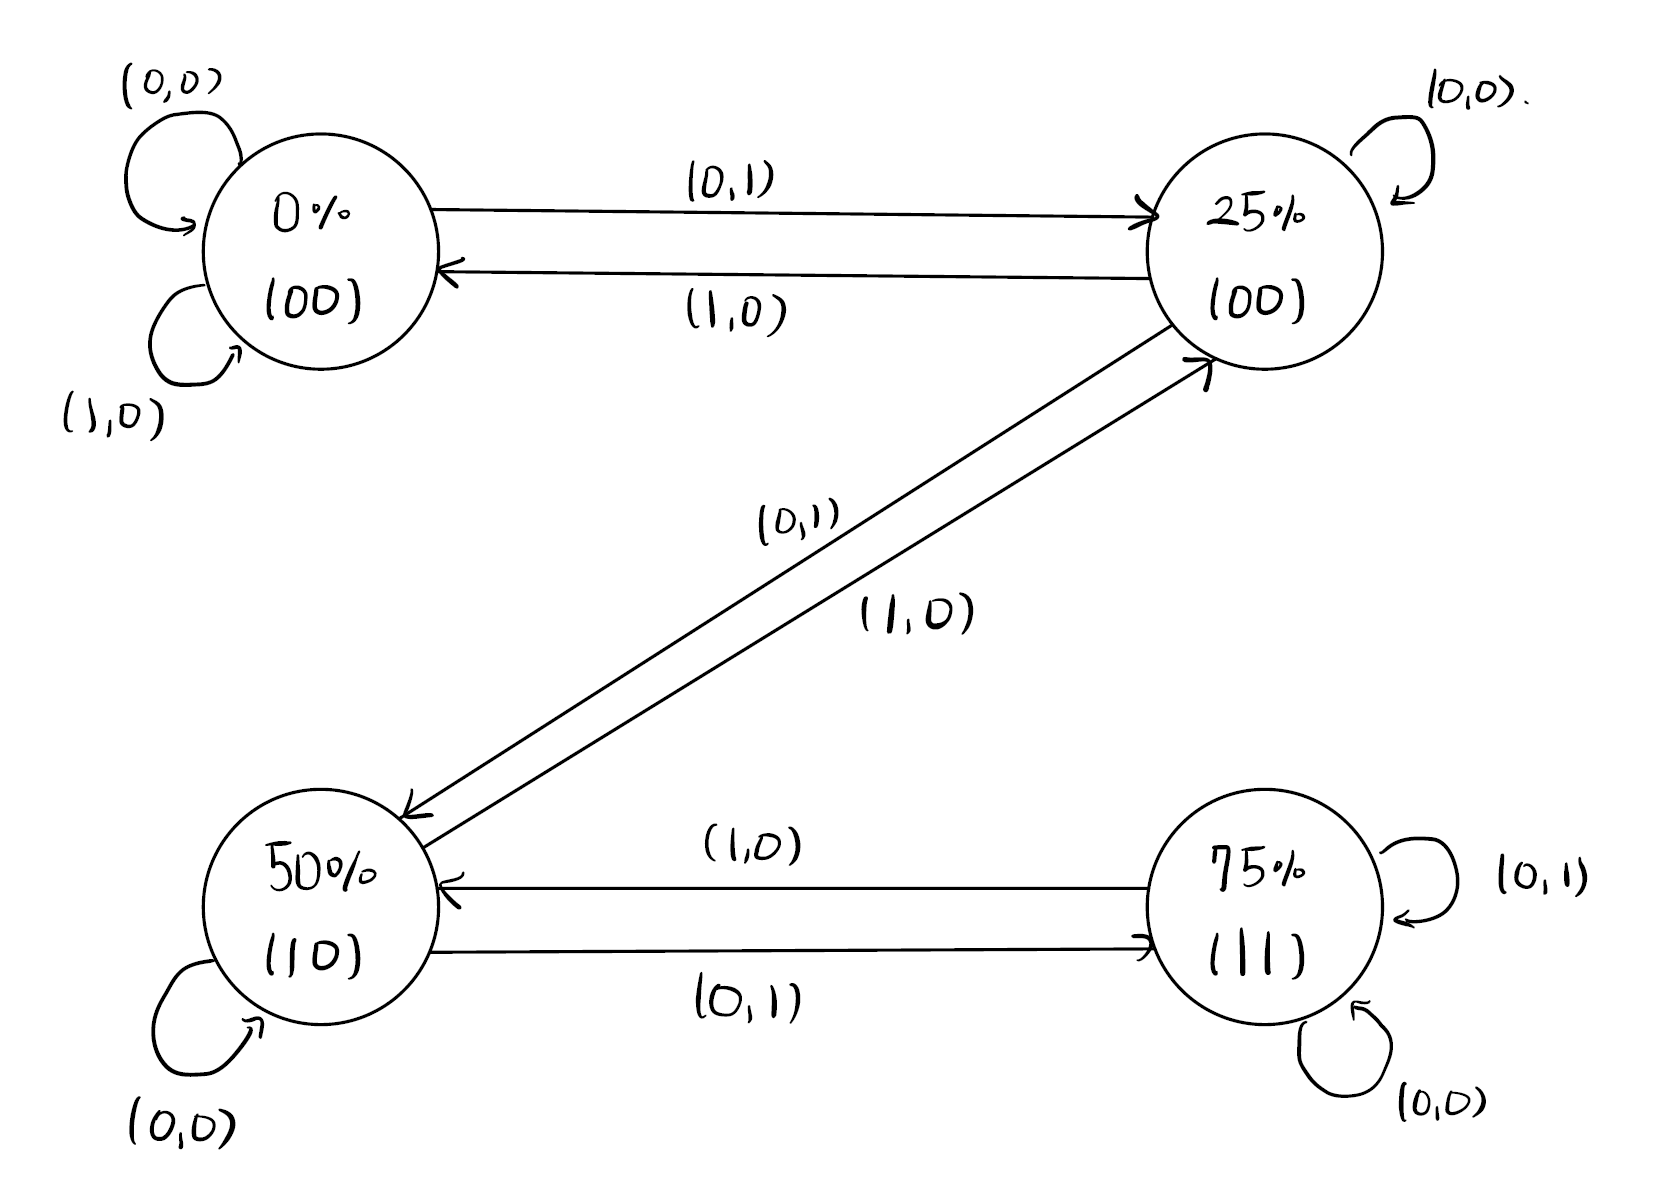
\includegraphics[width=.6\linewidth]{src/Part 1_State Machine Diagram.png}
    \caption{State Machine Diagram of Part I}
\end{figure}

\subsection*{(e) Logical Functional Expressions and Logic Circuit}
Figure 2 is the K-map of state variable $Q_1^*$. Figure 3 shows the K-map of state variable $Q_0^*$.
\begin{figure}[!ht]
    \centering
    \begin{minipage}{0.45\textwidth}
        \centering
        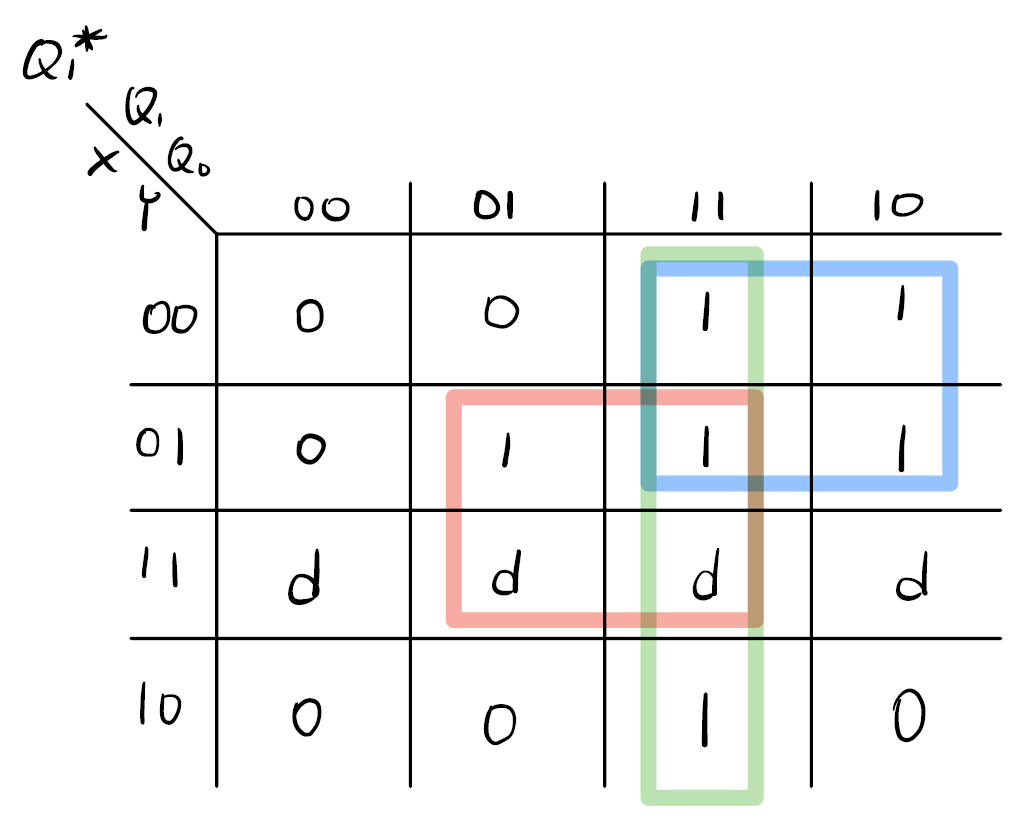
\includegraphics[width=.8\linewidth]{src/Part 1_Kmap_Q1.png}
        \caption{K-map of $Q_1^*$}
    \end{minipage}\hfill
    \begin{minipage}{0.45\textwidth}
        \centering
        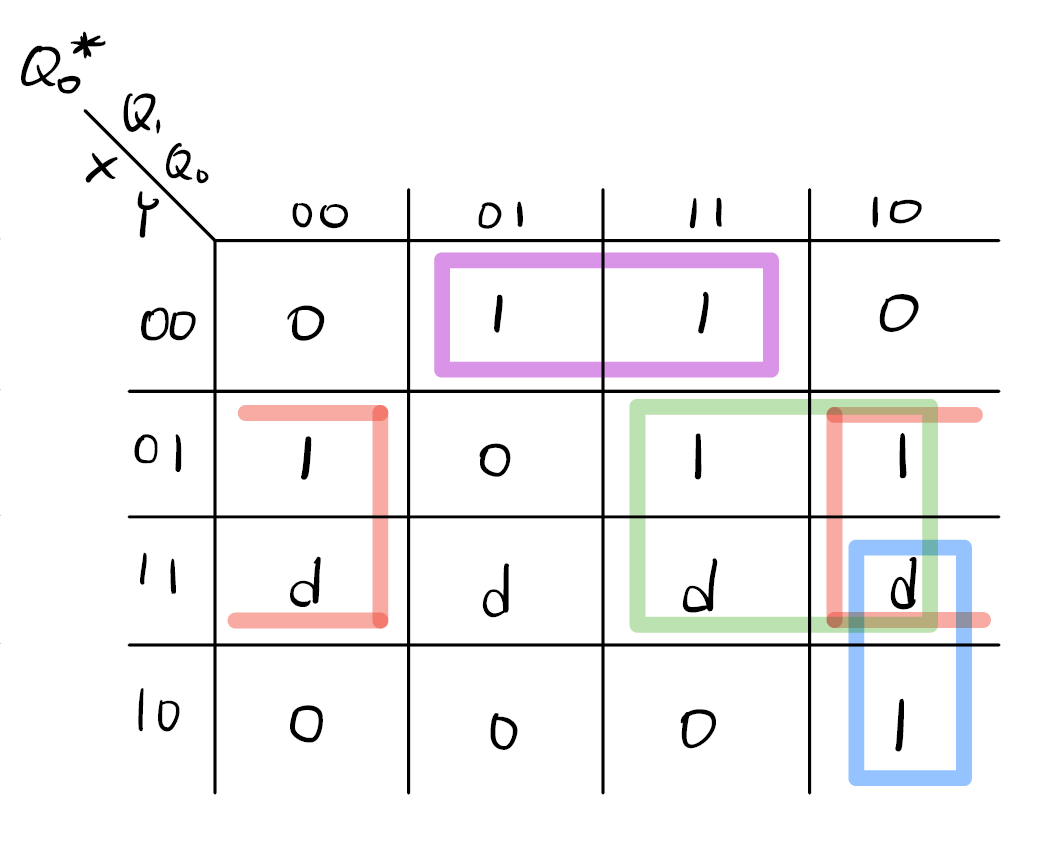
\includegraphics[width=.8\linewidth]{src/Part 1_Kmap_Q0.png}
        \caption{K-map of $Q_0^*$}
    \end{minipage}
\end{figure}

From above K-maps, we obtain the equations for $Q_1^*$ and $Q_0^*$:
\begin{equation}
    Q_1^* = Q_0 Y + Q_1 \overline{X} + Q_1 Q_0
\end{equation}
\begin{equation}
    Q_0^* = Y \overline{Q_0} + Y Q_1 + \overline{X} Q_0 \overline{Y} + X Q_1 \overline{Q_0}
\end{equation}

Using both equations, we can obtain the circuit by using two positive-edge triggered D Flip Flops for state variables $Q_0$ and $Q_1$. Figure 4 is the circuit diagram for part 1.
\begin{figure}[!ht]
    \centering
    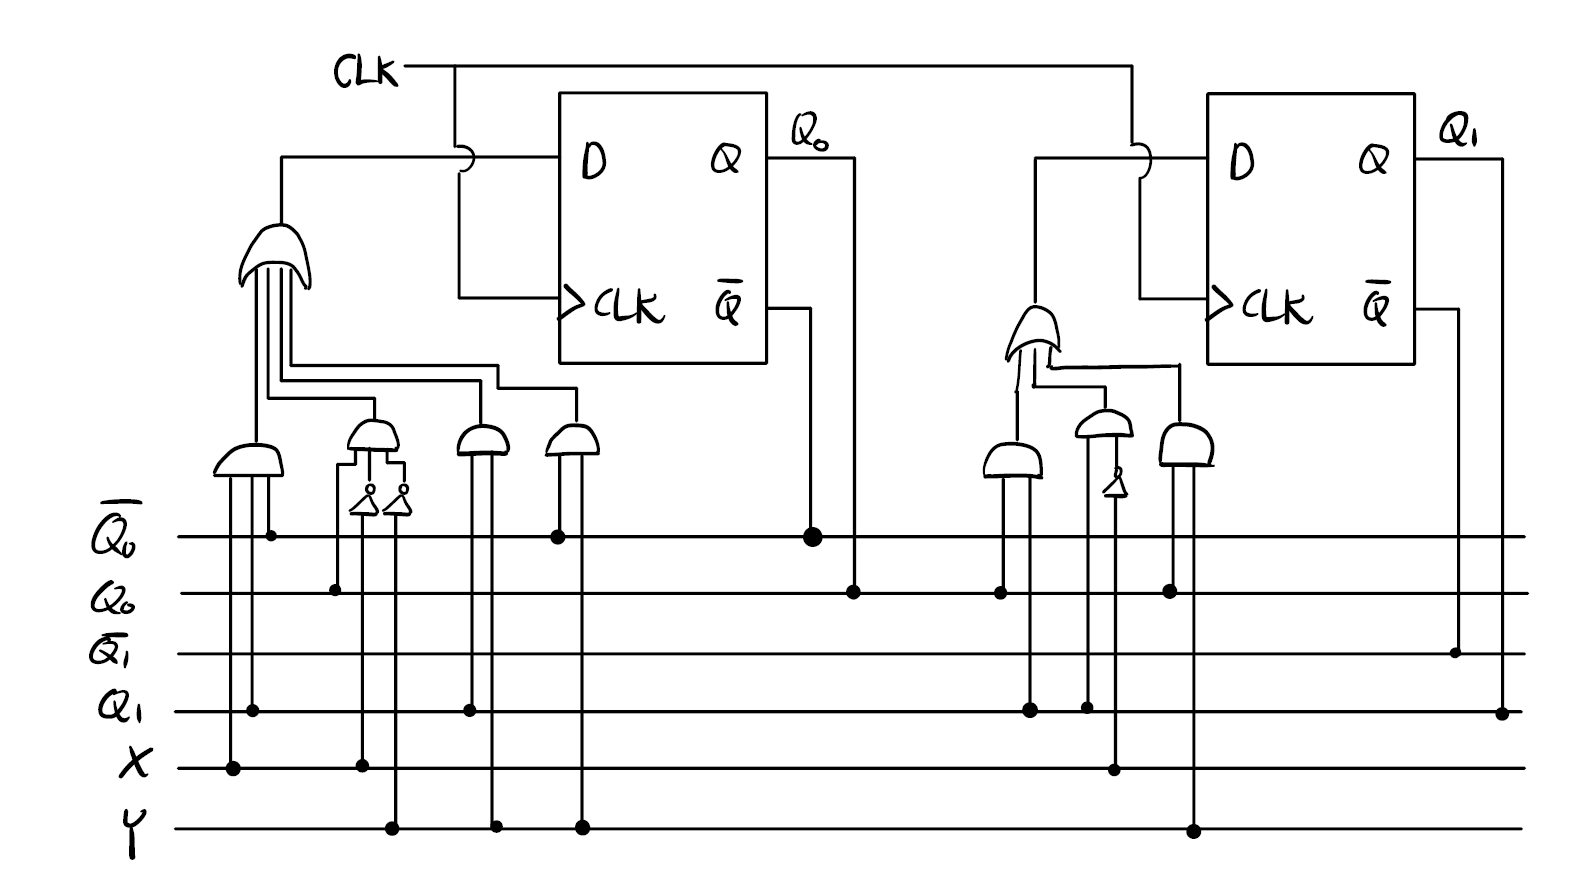
\includegraphics[width=.75\linewidth]{src/Part 1_Circuit Diagram.png}
    \caption{Circuit Diagram}
\end{figure}

\subsection*{(f) Design Restrictions}
If we did not incorporate the restrictions about these specific cases, then we will treat them as don't cares in our state transition table, corresponding K-map, and the equations. Having a don't care in truth table may result in a different circuit design which do not behave equally. This is okay if the input corresponding to those don't cares is invalid and never used while the user operates the circuit. In this example, input $I=XY=11$ is never used, so it's okay to put don't care signs. However, aforementioned situations from part (c) can possibly happen, meaning that we should be able to control these states. Without restrictions, we don't have a full control on these cases. This is a great obstacle where we should be able to expect every behavior of a circuit. Therefore, it was necessary to incorporate the restrictions from part (c).


\section*{Design of a switching power converter Part II}

\subsection*{(a) State Transition Table}
Current state is represented as $C_1C_0$. Next state and output are marked as ($C_1^*C_0^*$, $S$). Input, which is a duty cycle is a 2 bit binary number $d = d_1d_0$. For example, $d=d_1d_0=01$ means 25\% duty cycle.

\begin{table}[!ht]
    \centering
    \begin{tabular}{|c|clll|}
    \hline
    \multirow{2}{*}{\begin{tabular}[c]{@{}c@{}}Current State\\ ($C_1C_0$)\end{tabular}} & \multicolumn{4}{c|}{(Next State, Output) ($C_1^*C_0^*$, $S$)}                                         \\ \cline{2-5} 
                                                                                    & \multicolumn{1}{l|}{$d_1d_0=00$} & \multicolumn{1}{l|}{$d_1d_0=01$} & \multicolumn{1}{l|}{$d_1d_0=10$} & $d_1d_0=11$ \\ \hline
    00                                                                    & \multicolumn{1}{c|}{(01, 0)} & \multicolumn{1}{l|}{(01, 1)} & \multicolumn{1}{l|}{(01, 1)} & (01, 1) \\ \hline
    01                                                                      & \multicolumn{1}{c|}{(10, 0)} & \multicolumn{1}{l|}{(10, 0)} & \multicolumn{1}{l|}{(10, 1)} & (10, 1) \\ \hline
    10                                                                      & \multicolumn{1}{c|}{(11, 0)} & \multicolumn{1}{l|}{(11, 0)} & \multicolumn{1}{l|}{(11, 0)} & (11, 1) \\ \hline
    11                                                                      & \multicolumn{1}{c|}{(00, 0)} & \multicolumn{1}{l|}{(00, 0)} & \multicolumn{1}{l|}{(00, 0)} & (00, 0) \\ \hline
    \end{tabular}
    \caption{State Transition Table of Part II}
\end{table}

\subsection*{(b) State Machine Diagram}
Figure 5 is the state machine diagram corresponding to Table 2. Input $d_1d_0$ and output $S$ are interpreted as a tuple ($d_1$, $d_0$) / $S$. For example, (0, 1), (1, 1), (1, 0) / 1 with a single arrow means for inputs (0, 1), (1, 1), and (1, 0), the machine outputs 1 and all these go to the same next state.
\begin{figure}[!ht]
    \centering
    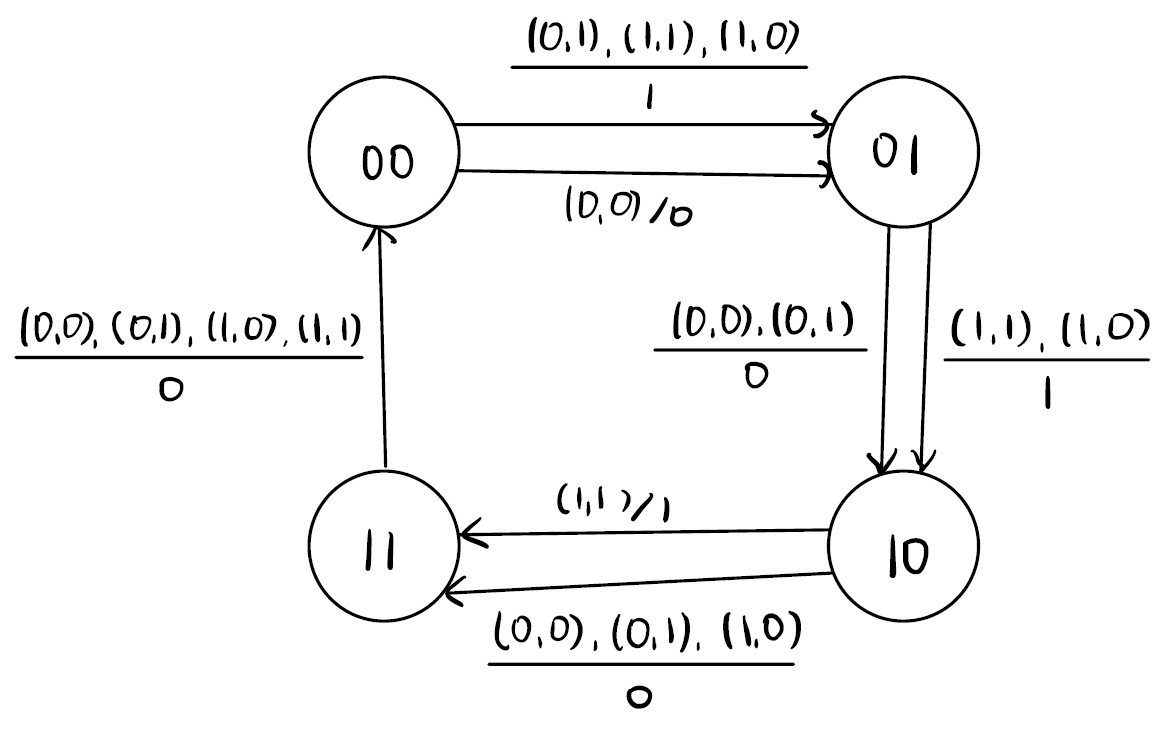
\includegraphics[width=.6\linewidth]{src/Part 2_State Machine Diagram.png}
    \caption{State Machine Diagram of Part II}
\end{figure}

\subsection*{(c) Logical Functional Expressions and Logic Circuit}
Figure 6 is the K-map of state variable $C_1^*$. Figure 7 is the K-map of state variable $C_0^*$.
\begin{figure}[!ht]
    \centering
    \begin{minipage}{0.45\textwidth}
        \centering
        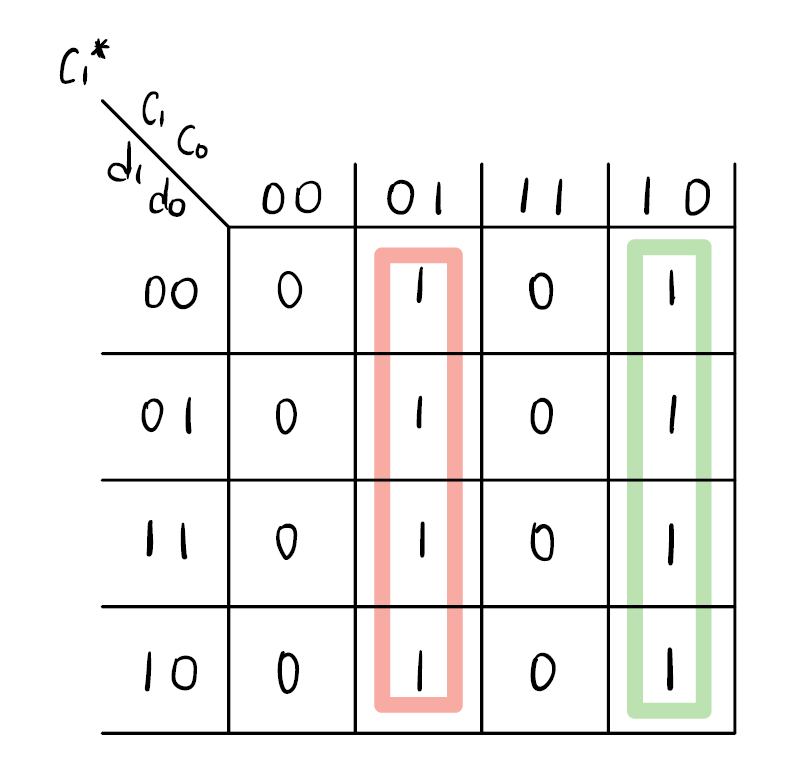
\includegraphics[width=.8\linewidth]{src/Part 2_Kmap_C1.png}
        \caption{K-map of $C_1^*$}
    \end{minipage}\hfill
    \begin{minipage}{0.45\textwidth}
        \centering
        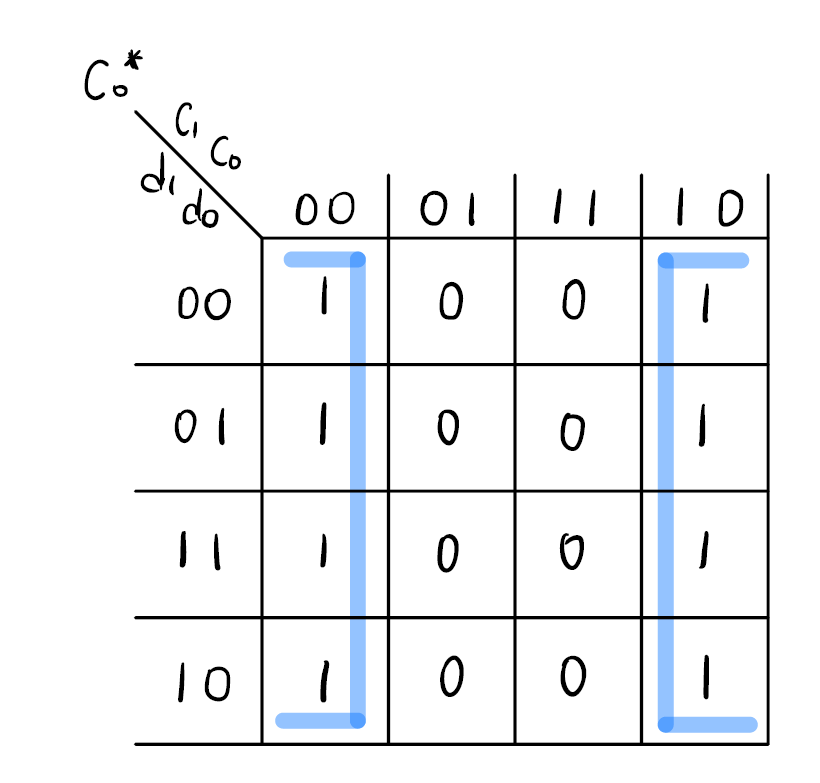
\includegraphics[width=.8\linewidth]{src/Part 2_Kmap_C0.png}
        \caption{K-map of $C_0^*$}
    \end{minipage}
\end{figure}

From those K-maps, we obtained the equation for $C_1^*$ and $C_0^*$.
\begin{equation}
    C_1^* = \overline{C_1} C_0 + C_1 \overline{C_0} = C_1 \oplus C_0
\end{equation}
\begin{equation}
    C_0^* = \overline{C_0}
\end{equation}

Finally, Figure 8 is the K-map of the output $S$.

\begin{figure}[!ht]
    \centering
    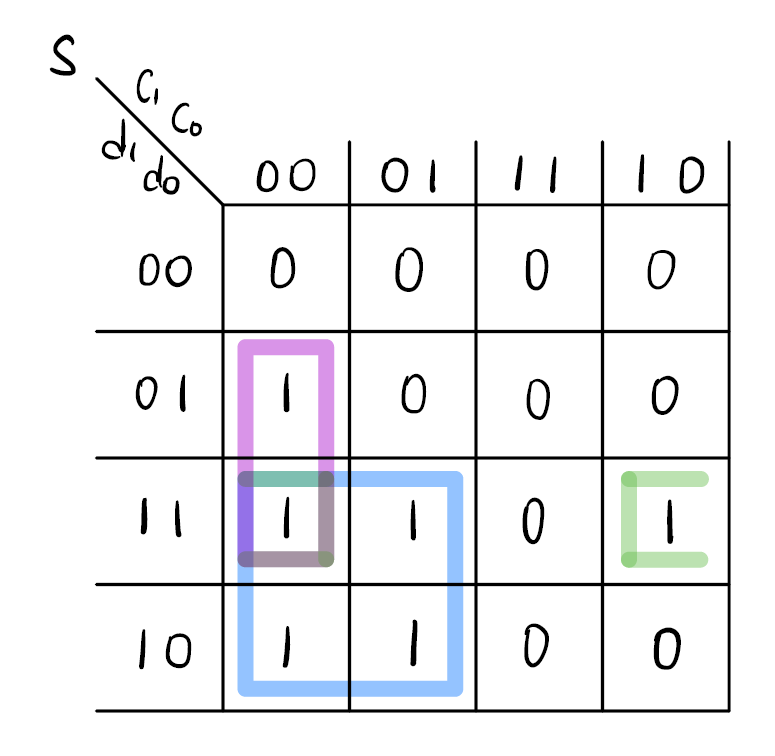
\includegraphics[width=.3\linewidth]{src/Part 2_Kmap_S.png}
    \caption{K-map of $S$}
\end{figure}

From the K-map, we obtained the equation for $S$:
\begin{equation}
    S = \overline{C_0} d_0 \overline{C_1} + \overline{C_0} d_1 d_0 + \overline{C_1} d_1 
\end{equation}
Using above three equations, we can obtain the logic circuit by using two positive-edge triggered D Flip Flops for state variables $C_0$ and $C_1$. Figure 9 is the circuit diagram for part 2.
\begin{figure}[!ht]
    \centering
    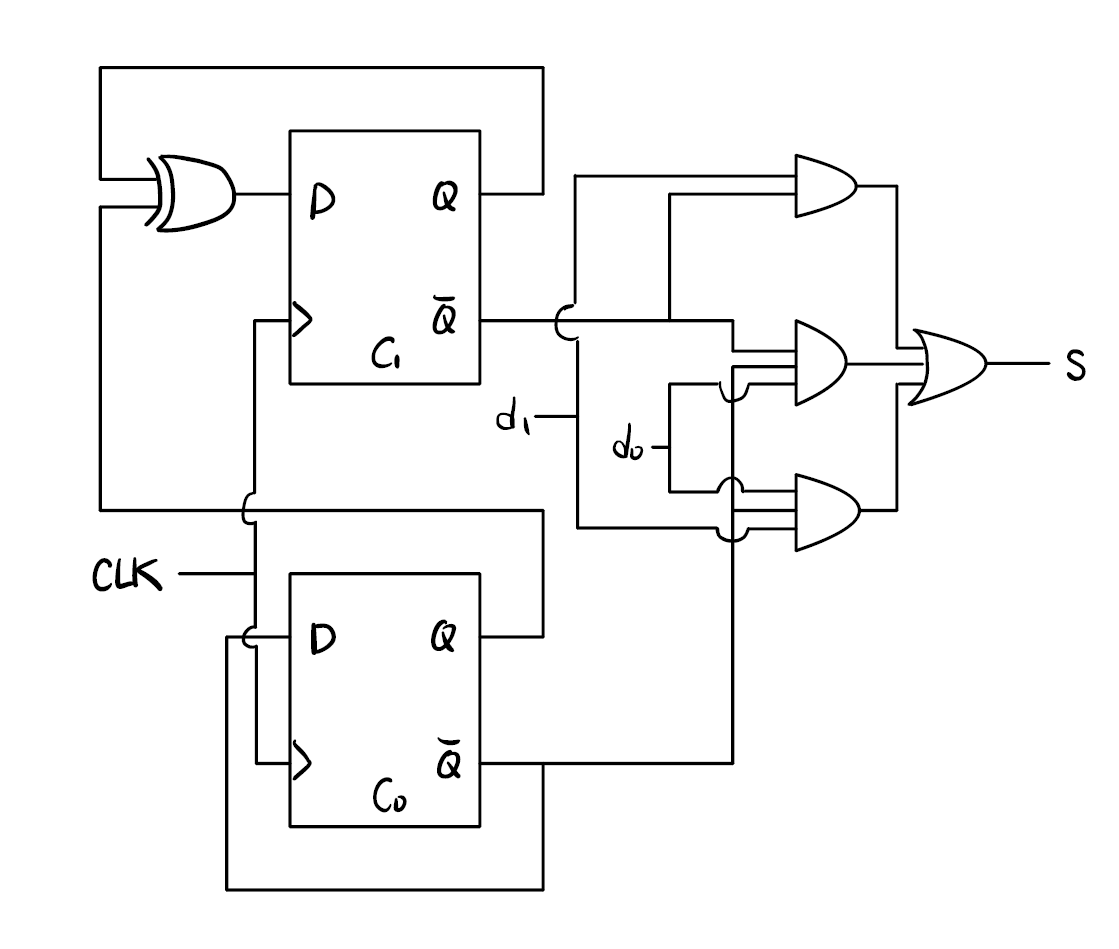
\includegraphics[width=.75\linewidth]{src/Part 2_Circuit Diagram.png}
    \caption{Circuit Diagram}
\end{figure}


\subsection*{(d) Timing Diagrams}
\subsubsection*{1. 25\% Duty Cycle}
Figure 10 shows the timing diagram for $S$ for duty cycle $d = d_1d_0 = 01 = 25\%$.
\begin{figure}[!ht]
    \centering
    \includegraphics*[width=.9\linewidth]{src/Timing_25.png}
    \caption{25\% Duty Cycle Timing Diagram for $S$}
\end{figure}

We observe that the $1:0$ ratio of the output signal $S$ is $1:3$, which is equivalent to the duty cycle of $\frac{1}{4} = 25\%$.

\subsubsection*{2. 75\% Duty Cycle}
Figure 11 shows the timing diagram for $S$ for duty cycle $d = d_1d_0 = 11 = 75\%$.
\begin{figure}[!ht]
    \centering
    \includegraphics*[width=.9\linewidth]{src/Timing_75.png}
    \caption{75\% Duty Cycle Timing Diagram for $S$}
\end{figure}

We observe that the $1:0$ ratio of the output signal $S$ is $3:1$, which is equivalent to the duty cycle of $\frac{3}{4} = 75\%$.


\subsection*{(e) Maximum Switching Frequency of the Converter}
Given the clock frequency of $1$MHz, the converter’s maximum switching frequency is $0.25$MHz.
The converter circuit is based on a 2-bit modulo counter. Therefore, a single switching cycle of $S$ depends on 4 clock cycles. Since the clock frequency is $1$MHz, the counter’s frequency can be at max of $\frac{1}{4} = 0.25$MHz.

Since flip flop is either positive or negative edge-triggered, each state variable $C_1$ and $C_0$ can switch at most $\frac{1}{2}$ the rate the clock signal changes. Therefore, after an entire clock cycle, state variables $C_1$ and $C_0$ can complete at most $\frac{1}{2}$ of its cycle. Since converter output $S$ depends on the state of both $C_1$ and $C_0$, the converter can switch at most $\frac{1}{4}$ of its cycle per clock cycle. This is equivalent to say that the maximum switching frequency of the converter is $1 \times \frac{1}{4} = 0.25$ MHz.

In general, given the clock frequency of $f_{clk}$ and $n$ number of bits, the counter’s maximum clock frequency $f_s$ is expressed as
\begin{equation}
f_s = \cfrac{f_{clk}}{2^n}
\end{equation}


\subsection*{(f) Design Tradeoff}
To design a circuit with a highly precise duty cycle, we need a counter with more bits, that is, $n$ increases in equation (6). As a result, $f_s$ decreases, meaning that the maximum clock frequency decreases, and the circuit becomes slower. Along with the speed issue, the circuit also consumes more energy and is expensive since a lot more gates resources are required.

Therefore, when the cost and resources are more important factors than precision and speed, it would be more efficient to have less precise duty cycles.

There is one example. Consider a desktop computer and a graphing calculator. We do not expect a desktop-level computing speed from a graphing calculator. Also, a calculator should prioritize its power management over the huge calculation speed or precision because it does not have a consistent power source; it runs on batteries. In this case, it would be wise to use less precise duty cycles for a graphing calculator.


\section*{Design of a switching power converter Part III}
\subsection*{(a) DEB Pin Information}
In my DEB-1002, I used pin IN1 and IN0 for input $d_1$ and $d_0$, respectively. For example, if I set (IN1, IN0) to (1, 0), the circuit will produce a corresponding waveform of 50\% duty cycle. \newline
Since DEB-1002 has a builtin clock signal, I set the CLOCK\_ENABLE to 1 and connected CLOCK pin to the inputs of my two positive edge triggered D Flip Flops(SN74HC74N). Finally, I used the pin OUT0 to demonstrate the working waveform.

\subsection*{(b) Circuit Implementation}
From the logical expressions obtained above, I made some changes to the final equation in order to reduce the complexity and required amount of gate resources.
\begin{equation}
    S = \overline{C_0} d_0 \overline{C_1} + \overline{C_0} d_1 d_0 + \overline{C_1} d_1 = \overline{C_0} d_0 (d_1 + \overline{C_1}) + \overline{C_1} d_1
\end{equation}
In total, I used 1 XOR, 2 OR, 3 AND gates. Also, I used 2 positive edge triggered D Flip Flops to store state variables. Figure 12 shows the circuit implementation in DEB-1002.
\begin{figure}[!ht]
    \centering
    \includegraphics*[width=.9\linewidth]{src/Final Circuit Implementation.jpg}
    \caption{Final Circuit Implementation}
\end{figure}

\subsection*{(c) Link to the Video Demo}
Here is the link to the video demo: \url{https://youtu.be/EXsVrjeMC9M}

\end{document}